\documentclass[12pt,a4paper]{article}

% ── Packages ──────────────────────────────────────────────────────────────
\usepackage[utf8]{inputenc}
\usepackage[T1]{fontenc}
\usepackage[english]{babel}
\usepackage{geometry}
\geometry{margin=2.5cm}
\usepackage{graphicx}
\usepackage{hyperref}
\hypersetup{
  colorlinks=true,
  linkcolor=blue!60!black,
  citecolor=blue!60!black,
  urlcolor=blue!60!black,
}
\usepackage{booktabs}
\usepackage{tabularx}
\usepackage{longtable}
\usepackage{enumitem}
\usepackage{listings}
\usepackage{xcolor}
\usepackage{tikz}
\usetikzlibrary{shapes.geometric, arrows.meta, positioning, fit, backgrounds, calc}
\usepackage{float}
\usepackage{caption}
\usepackage{amsmath}

% ── Listing style ─────────────────────────────────────────────────────────
\lstset{
  basicstyle=\ttfamily\small,
  backgroundcolor=\color{gray!8},
  frame=single,
  rulecolor=\color{gray!40},
  breaklines=true,
  keywordstyle=\color{blue!70!black}\bfseries,
  commentstyle=\color{green!50!black}\itshape,
  stringstyle=\color{red!60!black},
  showstringspaces=false,
  tabsize=2,
  columns=fullflexible,
}

% ── Title ─────────────────────────────────────────────────────────────────
\title{%
  \textbf{Stimmbandl\"asion Web Tool}\\[0.4em]
  \Large Architecture Documentation
}
\author{}
\date{\today}

% ══════════════════════════════════════════════════════════════════════════
\begin{document}
\maketitle
\tableofcontents
\newpage

% ══════════════════════════════════════════════════════════════════════════
\section{Introduction}
\label{sec:introduction}

The \emph{Stimmbandl\"asion} web tool is a medical data-collection platform for
vocal cord lesion (recurrent laryngeal nerve paresis) diagnosis. It manages
patient records, collects voice audio recordings for pre-operative and
post-operative phases, integrates an AI inference service for automated
prediction, and provides data export functionality for clinical research.

The application follows a containerised microservice architecture orchestrated
with Docker~Compose, comprising a Django REST back\-end, a React single-page
application front\-end, an Nginx reverse proxy, and supporting infrastructure
services (PostgreSQL, MinIO / S3, Redis).

% ══════════════════════════════════════════════════════════════════════════
\section{System Overview}
\label{sec:overview}

Figure~\ref{fig:system-overview} illustrates the high-level request flow and
service topology.

\begin{figure}[H]
\centering
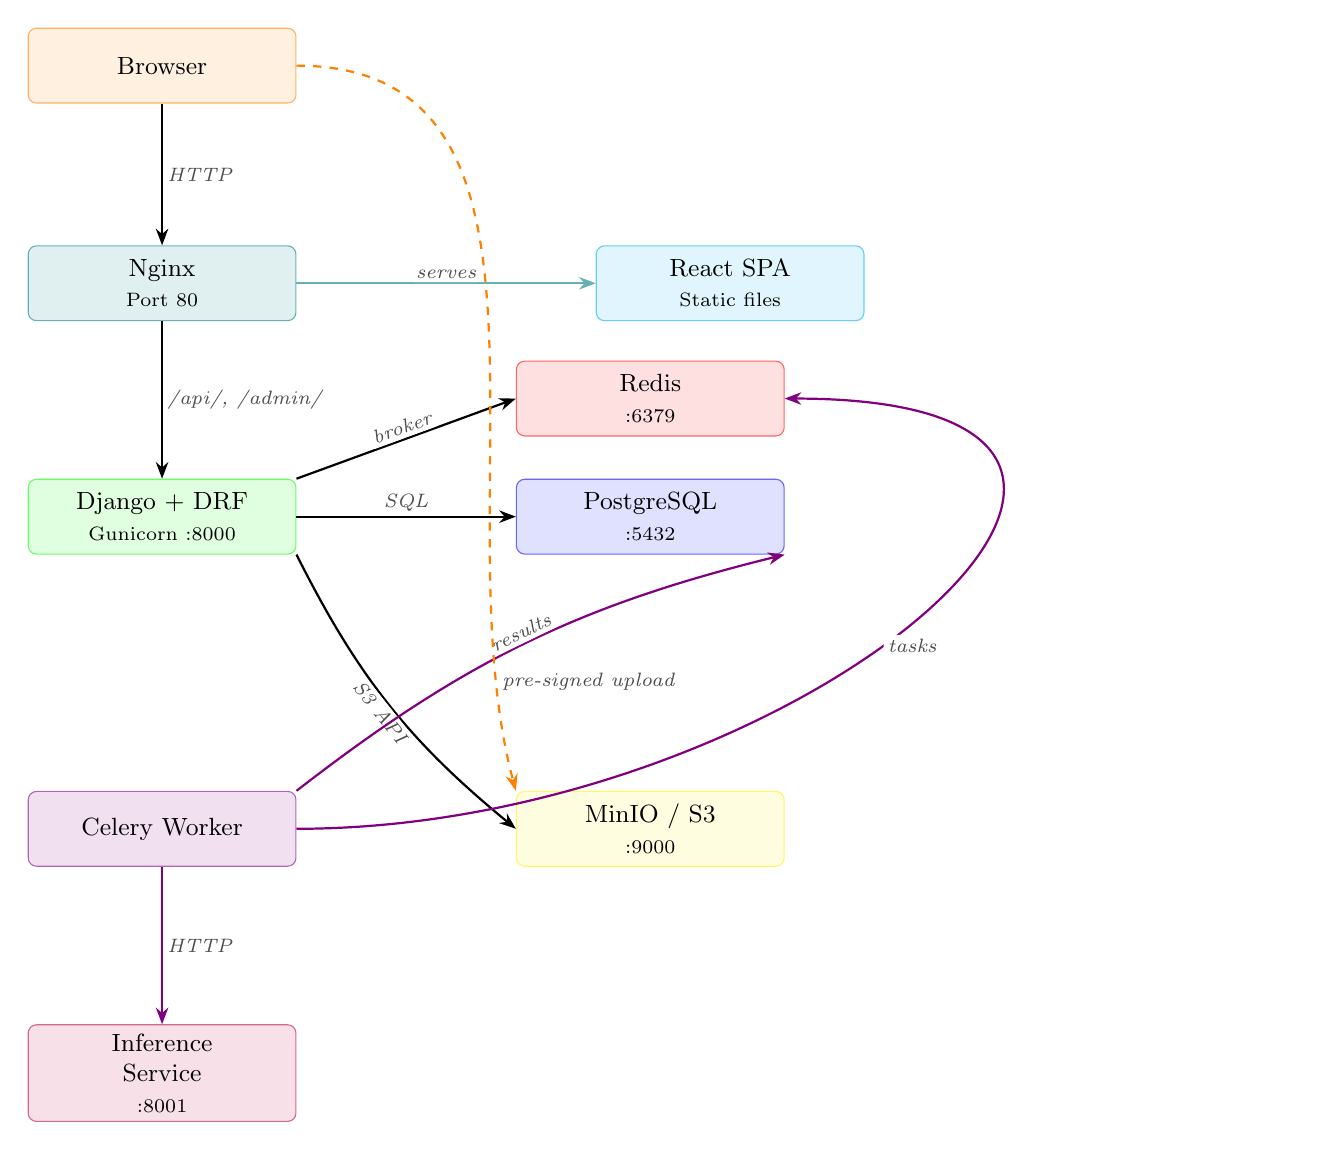
\begin{tikzpicture}[
    box/.style={
      rectangle, draw, rounded corners=3pt,
      minimum width=3.4cm, minimum height=0.95cm,
      font=\small, align=center,
      fill=#1!12, draw=#1!60
    },
    box/.default=blue,
    arr/.style={-{Stealth[length=6pt]}, thick, #1},
    arr/.default=black,
    lbl/.style={font=\scriptsize\itshape, text=gray!60!black,
                fill=white, inner sep=1.5pt, rounded corners=1pt},
  ]

  %% ── Vertical spine (left column, top → bottom) ────────────────────────
  \node[box=orange]  (browser)   {Browser};
  \node[box=teal,    below=1.8cm of browser]  (nginx)     {Nginx\\{\scriptsize Port 80}};
  \node[box=green,   below=2.0cm of nginx]    (django)    {Django + DRF\\{\scriptsize Gunicorn :8000}};
  \node[box=violet,  below=3.0cm of django]   (celery)    {Celery Worker};
  \node[box=purple,  below=2.0cm of celery]   (inference) {Inference\\Service\\{\scriptsize :8001}};

  %% ── React SPA (right of Nginx) ────────────────────────────────────────
  \node[box=cyan, right=3.8cm of nginx] (react) {React SPA\\{\scriptsize Static files}};

  %% ── Data layer (right column) ─────────────────────────────────────────
  %  Redis:  above django level (no crossing with django→pg)
  %  pg:     same level as django (straight horizontal arrow)
  %  MinIO:  same level as celery (straight horizontal arrow)
  \node[box=red]    (redis) at ($(django) + (6.2cm,  1.5cm)$) {Redis\\{\scriptsize :6379}};
  \node[box=blue]   (pg)    at ($(django) + (6.2cm,  0cm)$)   {PostgreSQL\\{\scriptsize :5432}};
  \node[box=yellow] (minio) at ($(celery) + (6.2cm,  0cm)$)   {MinIO / S3\\{\scriptsize :9000}};

  %% ── Spine arrows ──────────────────────────────────────────────────────
  \draw[arr]         (browser) -- node[right, lbl] {HTTP}           (nginx);
  \draw[arr]         (nginx)   -- node[right, lbl] {/api/, /admin/} (django);
  \draw[arr=teal!60] (nginx)   -- node[above, lbl] {serves}         (react);
  \draw[arr=violet]  (celery)  -- node[right, lbl] {HTTP}           (inference);

  %% ── Django → data layer ───────────────────────────────────────────────
  %  broker: gentle up-right to Redis
  \draw[arr] (django.north east)
      -- node[above, sloped, lbl] {broker} (redis.west);
  %  SQL: straight horizontal to PostgreSQL
  \draw[arr] (django.east)
      -- node[above, lbl] {SQL} (pg.west);
  %  S3 API: down-right to MinIO (bent slightly south to clear celery→pg)
  \draw[arr] (django.south east)
      to[bend right=12]
      node[below, sloped, lbl] {S3 API} (minio.west);

  %% ── Celery → data layer ───────────────────────────────────────────────
  %  tasks: loop out to the right of the data column, no crossings
  \draw[arr=violet] (celery.east)
      to[out=0, in=0, looseness=2.0]
      node[right, lbl, pos=0.45] {tasks} (redis.east);
  %  results: up-right to PostgreSQL (bent north to clear django→minIO)
  \draw[arr=violet] (celery.north east)
      to[bend left=12]
      node[above, sloped, lbl] {results} (pg.south east);

  %% ── Pre-signed upload (dashed) ────────────────────────────────────────
  \draw[arr=orange, dashed] (browser.east)
      to[out=0, in=105]
      node[right, lbl, pos=0.88] {pre-signed upload} (minio.north west);

\end{tikzpicture}
\caption{System overview and request flow.}
\label{fig:system-overview}
\end{figure}

% ══════════════════════════════════════════════════════════════════════════
\section{Technology Stack}
\label{sec:tech-stack}

\begin{table}[H]
\centering
\caption{Technology choices and rationale.}
\label{tab:tech-stack}
\begin{tabularx}{\textwidth}{l l X}
\toprule
\textbf{Concern} & \textbf{Choice} & \textbf{Rationale} \\
\midrule
Back-end framework   & Django 5.1 + DRF     & Mature ORM, built-in admin, serialisers, permissions \\
Front-end framework  & React 19 + Vite 8    & Fast builds, TypeScript, component model \\
UI component library & Material UI (MUI) 7  & Consistent design system, rich widget set \\
Reverse proxy        & Nginx                & Serves SPA static files, proxies API \\
WSGI server          & Gunicorn             & Production-grade, multi-worker \\
Database             & PostgreSQL 16        & Relational, robust, widely supported \\
Object storage       & MinIO (dev) / S3 (prod) & S3-compatible, self-hosted for development \\
Task queue           & Celery + Redis       & Asynchronous inference calls \\
Authentication       & JWT (SimpleJWT)      & Stateless admin auth; UUID tokens for patients \\
Containerisation     & Docker + Compose     & Reproducible, portable deployments \\
\bottomrule
\end{tabularx}
\end{table}

% ══════════════════════════════════════════════════════════════════════════
\section{Infrastructure and Deployment}
\label{sec:infrastructure}

\subsection{Docker Compose Services}

\hbox{All services are defined in \texttt{docker-compose.yml} with development}
overrides in \texttt{docker-compose.dev.yml}.

\begin{table}[H]
\centering
\caption{Docker Compose service definitions.}
\label{tab:docker-services}
\begin{tabularx}{\textwidth}{l l l X}
\toprule
\textbf{Service} & \textbf{Image} & \textbf{Port(s)} & \textbf{Role} \\
\midrule
\texttt{db}      & \texttt{postgres:16-alpine} & 5432 & Primary relational database \\
\texttt{minio}   & \texttt{minio/minio:latest} & 9000, 9001 & S3-compatible object storage (audio files) \\
\texttt{redis}   & \texttt{redis:7-alpine}     & 6379 & Celery message broker \\
\texttt{backend} & Custom (Python 3.12)        & 8000 & Django application server \\
\texttt{celery}  & Same as backend             & ---  & Asynchronous task worker \\
\texttt{nginx}   & Custom (nginx:alpine)       & 80   & Reverse proxy + SPA host \\
\bottomrule
\end{tabularx}
\end{table}

Three named Docker volumes persist data: \texttt{postgres\_data},
\texttt{minio\_data}, and \texttt{static\_files}.

\subsection{Nginx Reverse Proxy}
\label{sec:nginx}

Nginx serves four location blocks:

\begin{table}[H]
\centering
\caption{Nginx routing rules.}
\label{tab:nginx-routes}
\begin{tabularx}{\textwidth}{l X}
\toprule
\textbf{Location} & \textbf{Target} \\
\midrule
\texttt{/api/*}    & Proxy to Django back-end (\texttt{backend:8000}) \\
\texttt{/admin/*}  & Proxy to Django admin interface \\
\texttt{/static/*} & Serve Django collected static files \\
\texttt{/*}        & Serve React SPA with \texttt{try\_files} fallback to \texttt{index.html} \\
\bottomrule
\end{tabularx}
\end{table}

The maximum client body size is set to 50\,MB to accommodate audio file uploads.

\subsection{Development vs.\ Production}

\begin{itemize}[nosep]
  \item \textbf{Development}: The back-end uses Django's built-in
    \texttt{runserver} with \texttt{DEBUG=True}; source code is bind-mounted for
    hot-reload. The Nginx container is disabled (profile \texttt{production});
    the React dev server runs locally on port~5173 with a Vite proxy for
    \texttt{/api} requests.
  \item \textbf{Production}: Gunicorn serves the Django application behind
    Nginx. The React SPA is built at image-build time and embedded into the
    Nginx container. Security hardening is enabled (HSTS, secure cookies,
    \texttt{X-Frame-Options: DENY}).
\end{itemize}

\subsection{Build Pipeline}

Both the back-end and front-end Dockerfiles use multi-stage builds:

\begin{enumerate}[nosep]
  \item \textbf{Back-end}: A \texttt{python:3.12-slim} builder installs system
    dependencies and Python packages; the runner stage copies only the installed
    packages and application code, runs as a non-root \texttt{django} user.
  \item \textbf{Front-end / Nginx}: A \texttt{node:22-alpine} builder produces
    the Vite production bundle; the final \texttt{nginx:alpine} image copies the
    built \texttt{dist/} directory and the Nginx configuration.
\end{enumerate}

On container start-up, the back-end entrypoint script automatically runs
database migrations, loads exercise fixture data, creates a default superuser,
and collects static files before handing off to Gunicorn.

% ══════════════════════════════════════════════════════════════════════════
\section{Back-end Architecture}
\label{sec:backend}

The Django project follows a split-settings pattern
(\texttt{config/settings/\{base, development, production\}.py}) and contains a
single application: \texttt{patients}.

\subsection{Data Model}
\label{sec:data-model}

The domain model consists of three entities. Figure~\ref{fig:er} shows the
entity-relationship diagram.

\begin{figure}[H]
\centering
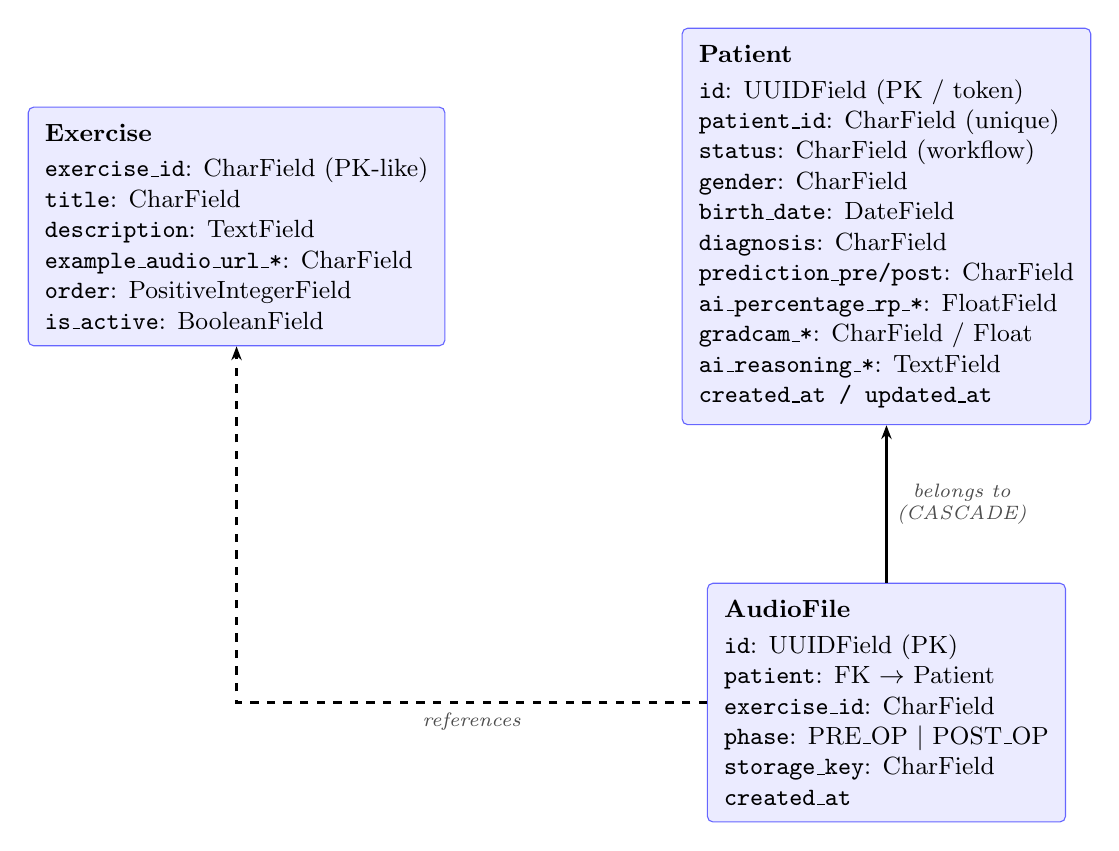
\begin{tikzpicture}[
    entity/.style={
      rectangle, draw=blue!60, fill=blue!8,
      rounded corners=2pt, minimum width=4.5cm,
      font=\small, align=left, inner sep=6pt
    },
    rel/.style={-{Stealth[length=5pt]}, thick},
    lbl/.style={font=\scriptsize\itshape, text=gray!60!black, align=center},
  ]

  \node[entity] (exercise) {
    \textbf{Exercise}\\[2pt]
    \texttt{exercise\_id}: CharField (PK-like)\\
    \texttt{title}: CharField\\
    \texttt{description}: TextField\\
    \texttt{example\_audio\_url\_*}: CharField\\
    \texttt{order}: PositiveIntegerField\\
    \texttt{is\_active}: BooleanField
  };

  \node[entity, right=3cm of exercise] (patient) {
    \textbf{Patient}\\[2pt]
    \texttt{id}: UUIDField (PK / token)\\
    \texttt{patient\_id}: CharField (unique)\\
    \texttt{status}: CharField (workflow)\\
    \texttt{gender}: CharField\\
    \texttt{birth\_date}: DateField\\
    \texttt{diagnosis}: CharField\\
    \texttt{prediction\_pre/post}: CharField\\
    \texttt{ai\_percentage\_rp\_*}: FloatField\\
    \texttt{gradcam\_*}: CharField / Float\\
    \texttt{ai\_reasoning\_*}: TextField\\
    \texttt{created\_at / updated\_at}
  };

  \node[entity, below=2.0cm of patient] (audio) {
    \textbf{AudioFile}\\[2pt]
    \texttt{id}: UUIDField (PK)\\
    \texttt{patient}: FK $\rightarrow$ Patient\\
    \texttt{exercise\_id}: CharField\\
    \texttt{phase}: PRE\_OP $|$ POST\_OP\\
    \texttt{storage\_key}: CharField\\
    \texttt{created\_at}
  };

  \draw[rel] (audio.north) -- node[right, lbl] {belongs to\\(CASCADE)} (patient.south);
  \draw[rel, dashed] (audio.west) -| node[below, lbl, pos=0.25] {references} (exercise.south);
\end{tikzpicture}
\caption{Entity-relationship diagram.}
\label{fig:er}
\end{figure}

\subsubsection{Patient Workflow States}

The \texttt{Patient.status} field encodes a linear workflow with the following
transitions:

\begin{center}
\small
\texttt{NEW} $\rightarrow$
\texttt{CONSENT\_GIVEN} $\rightarrow$
\texttt{DEMOGRAPHICS\_DONE} $\rightarrow$
\texttt{PRE\_OP\_DONE} $\rightarrow$
\texttt{POST\_OP\_STARTED} $\rightarrow$
\texttt{POST\_OP\_DONE} $\rightarrow$
\texttt{COMPLETED}
\end{center}

Each transition is enforced by the \texttt{advance\_patient\_step()} service
function, which also records timestamps (\texttt{pre\_op\_date},
\texttt{post\_op\_date}) and triggers asynchronous inference tasks at the
appropriate stages.

\subsubsection{Enumerations}

\begin{table}[H]
\centering
\caption{Model choice fields.}
\label{tab:enums}
\begin{tabular}{l p{9cm}}
\toprule
\textbf{Field} & \textbf{Values} \\
\midrule
\texttt{Patient.status}     & NEW, CONSENT\_GIVEN, DEMOGRAPHICS\_DONE,\\
                            & PRE\_OP\_DONE, POST\_OP\_STARTED, POST\_OP\_DONE, COMPLETED \\
\texttt{Patient.gender}     & M (male), W (female), D (diverse), ? (unknown) \\
\texttt{Patient.diagnosis}  & LEFT, RIGHT, BOTH, HEALTHY, TODO \\
\texttt{Patient.prediction\_*} & TODO, INFECTED, HEALTHY \\
\texttt{AudioFile.phase}    & PRE\_OP, POST\_OP \\
\bottomrule
\end{tabular}
\end{table}

\subsection{REST API}
\label{sec:api}

The API is built with Django REST Framework and split into three groups based on
authentication requirements.

\subsubsection{Authentication Endpoints}

\begin{table}[H]
\centering
\caption{JWT authentication endpoints.}
\begin{tabular}{l l l}
\toprule
\textbf{Method} & \textbf{URL} & \textbf{Description} \\
\midrule
POST & \texttt{/api/auth/token/}         & Obtain JWT access + refresh token \\
POST & \texttt{/api/auth/token/refresh/}  & Refresh an expired access token \\
\bottomrule
\end{tabular}
\end{table}

Access tokens expire after 2~hours; refresh tokens after 7~days and are rotated
and blacklisted upon use.

\subsubsection{Admin Endpoints (JWT Required)}

\begin{table}[H]
\centering
\caption{Admin API endpoints.}
\label{tab:admin-api}
\begin{tabularx}{\textwidth}{l l X}
\toprule
\textbf{Method} & \textbf{URL} & \textbf{Description} \\
\midrule
GET    & \texttt{/api/patients/}                  & List all patients (paginated) \\
POST   & \texttt{/api/patients/}                  & Create new patient \\
GET    & \texttt{/api/patients/\{id\}/}            & Retrieve patient details \\
PATCH  & \texttt{/api/patients/\{id\}/}            & Update patient fields \\
DELETE & \texttt{/api/patients/\{id\}/}            & Delete patient and S3 files \\
POST   & \texttt{/api/patients/\{id\}/advance/}    & Advance workflow step \\
GET    & \texttt{/api/patients/\{id\}/completeness/} & Check data completeness \\
GET    & \texttt{/api/patients/\{id\}/pdf/}        & Download QR-code PDF \\
GET    & \texttt{/api/export/}                     & Export CSV + audio ZIP \\
\bottomrule
\end{tabularx}
\end{table}

\subsubsection{Patient-Facing Endpoints (UUID Token)}

These endpoints use the patient's UUID primary key as an access token embedded
in QR codes, requiring no separate authentication.

\begin{table}[H]
\centering
\caption{Patient-facing API endpoints.}
\label{tab:patient-api}
\begin{tabularx}{\textwidth}{l l X}
\toprule
\textbf{Method} & \textbf{URL} & \textbf{Description} \\
\midrule
GET  & \texttt{/api/p/\{token\}/}              & Get public patient data \\
PATCH & \texttt{/api/p/\{token\}/}             & Update demographics \\
POST & \texttt{/api/p/\{token\}/advance/}      & Advance workflow step \\
POST & \texttt{/api/p/\{token\}/audio/upload/}  & Upload audio file (server-side) \\
POST & \texttt{/api/p/\{token\}/audio/presign/} & Obtain pre-signed upload URL \\
POST & \texttt{/api/p/\{token\}/audio/confirm/} & Confirm pre-signed upload \\
\bottomrule
\end{tabularx}
\end{table}

\subsubsection{Public Endpoints}

\begin{table}[H]
\centering
\caption{Public API endpoints.}
\begin{tabularx}{\textwidth}{l l X}
\toprule
\textbf{Method} & \textbf{URL} & \textbf{Description} \\
\midrule
GET & \texttt{/api/exercises/}        & List active voice exercises \\
GET & \texttt{/api/audio/\{id\}/}     & Stream audio file from S3 \\
GET & \texttt{/api/audio/\{id\}/url/} & Pre-signed download URL (JWT) \\
\bottomrule
\end{tabularx}
\end{table}

\subsection{Serialisers}

DRF serialisers control field exposure and validation:

\begin{table}[H]
\centering
\caption{DRF serialiser classes.}
\label{tab:serialisers}
\begin{tabularx}{\textwidth}{l X}
\toprule
\textbf{Serialiser} & \textbf{Purpose} \\
\midrule
\texttt{PatientListSerializer}      & Compact list view with computed \texttt{audio\_count\_pre/post} \\
\texttt{PatientDetailSerializer}    & Full detail with nested audio files, age computation \\
\texttt{PatientPublicSerializer}    & Restricted view omitting AI and sensitive fields \\
\texttt{PatientCreateSerializer}    & Accepts only \texttt{patient\_id} with uniqueness validation \\
\texttt{PatientUpdateSerializer}    & Demographics, diagnosis, and AI result fields \\
\texttt{ExerciseSerializer}         & Read-only exercise metadata \\
\texttt{AudioFileSerializer}        & Full audio file metadata (admin) \\
\texttt{AudioFileCompactSerializer} & Compact audio metadata \\
\texttt{CompletenessSerializer}     & Boolean \texttt{complete}, lists of \texttt{missing}/\texttt{warnings} \\
\bottomrule
\end{tabularx}
\end{table}

\subsection{Permissions}

\begin{table}[H]
\centering
\caption{Custom DRF permission classes.}
\begin{tabularx}{\textwidth}{l X}
\toprule
\textbf{Class} & \textbf{Logic} \\
\midrule
\texttt{IsAdminUser}          & Requires JWT-authenticated user \\
\texttt{IsPatientTokenValid}  & Validates UUID token in URL maps to existing patient \\
\texttt{IsAdminOrPatientToken}& Allows access with either JWT or valid patient token \\
\bottomrule
\end{tabularx}
\end{table}

\subsection{Business Logic Services}
\label{sec:services}

Domain logic is centralised in \texttt{patients/services.py}:

\begin{table}[H]
\centering
\caption{Service layer functions.}
\label{tab:services}
\begin{tabularx}{\textwidth}{l X}
\toprule
\textbf{Function} & \textbf{Description} \\
\midrule
\texttt{advance\_patient\_step()} & State machine enforcing valid workflow transitions; sets timestamps and triggers inference tasks \\
\texttt{check\_completeness()}    & Validates that all required demographics, diagnosis, and audio files are present \\
\texttt{generate\_patient\_pdf()} & Produces a PDF with a QR code linking to the patient wizard \\
\texttt{export\_patients\_zip()}  & Generates a ZIP archive containing a CSV summary and all audio files for completed patients \\
\texttt{delete\_patient\_with\_files()} & Deletes S3 objects before cascading the database delete \\
\texttt{generate\_presigned\_upload\_url()} & Creates a pre-signed S3 PUT URL for direct client-to-storage uploads \\
\texttt{generate\_presigned\_download\_url()} & Creates a pre-signed S3 GET URL \\
\texttt{upload\_audio\_to\_s3()}  & Server-side upload of audio data to S3 \\
\texttt{get\_audio\_from\_s3()}   & Downloads audio bytes from S3 \\
\bottomrule
\end{tabularx}
\end{table}

\subsection{Asynchronous Tasks}
\label{sec:celery}

Celery is configured with a Redis broker and \texttt{django-db} result
back-end. A single shared task is defined:

\begin{description}[nosep]
  \item[\texttt{run\_inference\_task(patient\_id, phase)}] Calls the external
    inference service at \texttt{/predict} and \texttt{/reasoning} endpoints.
    The payload includes the S3 bucket, audio file keys, patient gender, and
    age. Results (prediction label, confidence percentage, Grad-CAM outputs,
    reasoning text) are stored back on the \texttt{Patient} model. The task
    retries up to 3~times with a 30-second delay.
\end{description}

\subsection{Dependencies}

Key Python packages (from \texttt{requirements.txt}):

\noindent
\begin{minipage}[t]{0.48\textwidth}
\begin{itemize}[nosep]
  \item Django $\geq$\,5.1
  \item djangorestframework $\geq$\,3.15
  \item djangorestframework-simplejwt $\geq$\,5.3
  \item django-cors-headers $\geq$\,4.4
  \item django-filter $\geq$\,24.0
  \item django-storages[s3] $\geq$\,1.14
  \item boto3 $\geq$\,1.35
\end{itemize}
\end{minipage}%
\hfill
\begin{minipage}[t]{0.48\textwidth}
\begin{itemize}[nosep]
  \item celery[redis] $\geq$\,5.4
  \item django-celery-results $\geq$\,2.5
  \item gunicorn $\geq$\,22.0
  \item psycopg2-binary $\geq$\,2.9
  \item reportlab $\geq$\,4.2
  \item qrcode[pil] $\geq$\,8.0
  \item requests $\geq$\,2.32
\end{itemize}
\end{minipage}

% ══════════════════════════════════════════════════════════════════════════
\section{Front-end Architecture}
\label{sec:frontend}

The front-end is a React 19 single-page application scaffolded with Vite~8 and
written in TypeScript. It uses Material UI (MUI)~7 for the component library and
Axios for HTTP communication.

\subsection{Routing}

\begin{table}[H]
\centering
\caption{Client-side routes.}
\label{tab:routes}
\begin{tabularx}{\textwidth}{l l l X}
\toprule
\textbf{Path} & \textbf{Component} & \textbf{Auth} & \textbf{Description} \\
\midrule
\texttt{/login}           & \texttt{LoginPage}          & Public    & Admin login form \\
\texttt{/}                & \texttt{DashboardPage}      & Protected & Patient list, create, export \\
\texttt{/details/:token}  & \texttt{PatientDetailsPage} & Protected & Full patient detail view \\
\texttt{/p/:token}        & \texttt{PatientWizardPage}  & Public    & Patient-facing data collection wizard \\
\bottomrule
\end{tabularx}
\end{table}

Protected routes check for a valid JWT in \texttt{localStorage} and redirect to
\texttt{/login} if absent.

\subsection{API Client}

Two Axios instances are configured in \texttt{src/api/client.ts}:

\begin{itemize}[nosep]
  \item \textbf{\texttt{api}} --- Admin requests with an interceptor that
    attaches the JWT \texttt{Bearer} token and automatically refreshes expired
    access tokens via the refresh endpoint.
  \item \textbf{\texttt{publicApi}} --- Unauthenticated requests for the
    patient-facing wizard flow.
\end{itemize}

Token lifecycle functions (\texttt{setTokens}, \texttt{clearTokens},
\texttt{isLoggedIn}) use \texttt{localStorage} keys \texttt{access\_token} and
\texttt{refresh\_token}.

\subsection{Patient Wizard Flow}
\label{sec:wizard}

The patient-facing wizard renders different screen components based on the
current \texttt{status} value:

\begin{figure}[H]
\centering
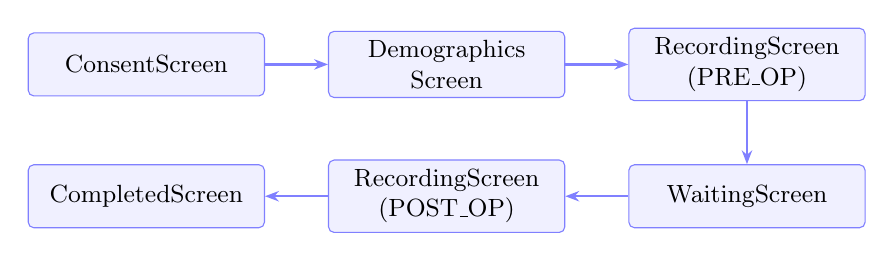
\begin{tikzpicture}[
    wizstep/.style={
      rectangle, draw=blue!50, fill=blue!6,
      rounded corners=2pt, minimum width=3.0cm, minimum height=0.8cm,
      font=\small, align=center
    },
    arr/.style={-{Stealth[length=5pt]}, thick, blue!50},
  ]

  \node[wizstep] (s1) {ConsentScreen};
  \node[wizstep, right=0.8cm of s1] (s2) {Demographics\\Screen};
  \node[wizstep, right=0.8cm of s2] (s3) {RecordingScreen\\(PRE\_OP)};
  \node[wizstep, below=0.8cm of s3] (s4) {WaitingScreen};
  \node[wizstep, left=0.8cm of s4] (s5) {RecordingScreen\\(POST\_OP)};
  \node[wizstep, left=0.8cm of s5] (s6) {CompletedScreen};

  \draw[arr] (s1) -- (s2);
  \draw[arr] (s2) -- (s3);
  \draw[arr] (s3) -- (s4);
  \draw[arr] (s4) -- (s5);
  \draw[arr] (s5) -- (s6);
\end{tikzpicture}
\caption{Patient wizard screen flow.}
\label{fig:wizard}
\end{figure}

\begin{table}[H]
\centering
\caption{Wizard screen--status mapping.}
\begin{tabular}{l l}
\toprule
\textbf{Patient Status} & \textbf{Screen Component} \\
\midrule
\texttt{NEW}              & \texttt{ConsentScreen} \\
\texttt{CONSENT\_GIVEN}   & \texttt{DemographicsScreen} \\
\texttt{DEMOGRAPHICS\_DONE} & \texttt{RecordingScreen} (phase = PRE\_OP) \\
\texttt{PRE\_OP\_DONE}    & \texttt{WaitingScreen} \\
\texttt{POST\_OP\_STARTED} & \texttt{RecordingScreen} (phase = POST\_OP) \\
\texttt{POST\_OP\_DONE / COMPLETED} & \texttt{CompletedScreen} \\
\bottomrule
\end{tabular}
\end{table}

\subsection{Audio Recording}

The \texttt{AudioRecorder} component uses the browser \texttt{MediaRecorder} API
to capture voice samples. Key features include:

\begin{itemize}[nosep]
  \item Real-time waveform visualisation via the \texttt{AudioVisualizer}
    component.
  \item Recording timer display.
  \item Playback of the recorded sample before submission.
  \item Example audio playback (male/female reference recordings).
  \item Audio quality validation: RMS level is computed in dBFS via the Web
    Audio API (\texttt{AudioContext}), with acceptance thresholds between
    $-30$\,dBFS and $-6$\,dBFS.
\end{itemize}

The \texttt{useExerciseSession} hook orchestrates the recording session: it
loads the exercise list from the API, manages the current exercise index, and
handles sequential upload and workflow advancement.

\subsection{Component Overview}

\begin{table}[H]
\centering
\caption{Key front-end components.}
\label{tab:components}
\begin{tabularx}{\textwidth}{l X}
\toprule
\textbf{Component} & \textbf{Description} \\
\midrule
\texttt{PatientList}         & Sortable, filterable MUI data table with search, status / diagnosis / prediction filters \\
\texttt{CreatePatientDialog} & Modal dialog to create a new patient record \\
\texttt{PatientAccessDialog} & Displays the patient access link and QR code \\
\texttt{AudioRecorder}       & Audio capture with waveform visualisation and quality checks \\
\texttt{AudioVisualizer}     & Real-time waveform rendering \\
\texttt{ConfirmDialog}       & Generic confirmation dialog \\
\texttt{StatusBadge}         & MUI Chip displaying workflow status with colour coding \\
\texttt{DiagnosisBadge}      & MUI Chip for diagnosis values \\
\texttt{PredictionBadge}     & MUI Chip for AI prediction results \\
\bottomrule
\end{tabularx}
\end{table}

\subsection{Theme}

The application uses a custom MUI theme with primary colour
\texttt{\#1565c0}, secondary colour \texttt{\#f57c00}, and a light background
(\texttt{\#f0f4f8}) using the Roboto typeface.

% ══════════════════════════════════════════════════════════════════════════
\section{Audio Upload Flow}
\label{sec:audio-upload}

Two upload strategies are supported to accommodate different deployment
scenarios:

\begin{enumerate}[nosep]
  \item \textbf{Server-side upload}: The audio blob is sent as
    \texttt{multipart/form-data} to the Django back-end, which writes it to
    S3/MinIO. This is simpler but routes all data through the application
    server.
  \item \textbf{Pre-signed URL upload}: The client requests a pre-signed S3 PUT
    URL from the back-end, uploads the file directly to MinIO/S3, and then
    confirms the upload. This bypasses Django for the actual file transfer,
    reducing server load.
\end{enumerate}

In both cases, an \texttt{AudioFile} database record is created linking the
patient, exercise, phase, and S3 storage key.

% ══════════════════════════════════════════════════════════════════════════
\section{AI Inference Integration}
\label{sec:inference}

After the pre-operative (or post-operative) recording phase is completed, the
\texttt{advance\_patient\_step()} function dispatches a Celery task
(\texttt{run\_inference\_task}) that:

\begin{enumerate}[nosep]
  \item Collects the S3 keys for all audio files of the relevant phase.
  \item Sends a prediction request to the external inference service at
    \texttt{\{INFERENCE\_SERVICE\_URL\}/predict} with the audio storage keys,
    patient gender, and age.
  \item Sends a reasoning request to \texttt{/reasoning} for explainability
    outputs.
  \item Stores the results on the \texttt{Patient} model: prediction label
    (\texttt{INFECTED}/\texttt{HEALTHY}), confidence percentage, Grad-CAM
    prediction and percentage, and reasoning text.
\end{enumerate}

The task is configured with automatic retries (up to 3 attempts, 30-second
delay) to handle transient inference service failures.

% ══════════════════════════════════════════════════════════════════════════
\section{Data Export}
\label{sec:export}

The export endpoint (\texttt{GET /api/export/}) generates a ZIP archive
containing:

\begin{itemize}[nosep]
  \item \textbf{\texttt{export.csv}}: A CSV file with all completed patient
    records including demographics, diagnosis, AI prediction results, and
    timestamps.
  \item \textbf{Audio files}: All associated audio recordings downloaded from
    S3, organised by patient and phase.
\end{itemize}

This supports offline analysis and integration with external research tools.

% ══════════════════════════════════════════════════════════════════════════
\section{Security Considerations}
\label{sec:security}

\begin{itemize}[nosep]
  \item \textbf{Authentication}: Admin routes require JWT tokens (access +
    refresh). Patient-facing routes are secured by unguessable UUID tokens
    embedded in QR codes.
  \item \textbf{CORS}: Allowed origins are configurable via environment
    variables; in production, only the application domain is permitted.
  \item \textbf{Production hardening}: HSTS is enabled, cookies are marked
    secure and HTTP-only, \texttt{X-Frame-Options} is set to \texttt{DENY}.
  \item \textbf{SQL injection}: Mitigated by Django ORM parameterised queries.
  \item \textbf{CSRF/XSS}: Django's built-in middleware active; DRF uses
    session-safe authentication classes.
  \item \textbf{File uploads}: Maximum body size enforced at the Nginx level
    (50\,MB); audio files are stored in isolated S3 buckets, not on the
    application filesystem.
  \item \textbf{Non-root containers}: The back-end runs as a dedicated
    \texttt{django} user inside the container.
\end{itemize}

% ══════════════════════════════════════════════════════════════════════════
\section{Summary}
\label{sec:summary}

The Stimmbandl\"asion web tool provides a complete clinical data-collection
pipeline: clinicians create patient records via an authenticated dashboard,
patients complete a guided wizard to provide demographic information and voice
recordings, an AI inference service analyses the recordings asynchronously, and
all data can be exported for research purposes. The fully containerised
architecture ensures reproducible deployments across development and production
environments.

\end{document}